% Generated by study2b/scripts/make_paper_results_2b.py from the committed analysis outputs.
% Do not edit by hand: change the script and re-run it.

\section{Results}
\label{sec:results}

Sections~\ref{sec:results-rq1} and~\ref{sec:results-rq2} answer RQ1 and RQ2 with the planned Study~2. Sections~\ref{sec:results-formfit} to~\ref{sec:results-2b-human} are exploratory: Section~\ref{sec:results-formfit} re-scores the exploratory Study~1 for RQ3, Section~\ref{sec:results-posthoc} is post hoc, and Section~\ref{sec:results-2b-human} reports the human ratings. Table~\ref{tab:claims} gives the status of each main claim.

\begin{table}
  \caption{Main claims and their status.}
  \label{tab:claims}
  \footnotesize
  \setlength{\tabcolsep}{3pt}
  \begin{tabular}{@{}>{\raggedright\arraybackslash}p{0.58\linewidth}cll@{}}
    \toprule
    Claim & Study & Status & Sect. \\
    \midrule
    Examples, rules and reasoning raise pattern fit & 2 & planned & \ref{sec:results-rq1} \\
    The effects of examples and reasoning differ between tiers & 2 & planned & \ref{sec:results-rq2} \\
    Examples help more than rules or native reasoning (on average over tiers) & 2 & post hoc & \ref{sec:results-rq1} \\
    Native reasoning helps more than written reasoning & 2 & post hoc & \ref{sec:results-rq1} \\
    Checker compliance alone would rank rules above examples & 2 & descriptive & \ref{sec:results-rq1} \\
    Form-only scoring changes which ingredients seem to matter & 1 & exploratory & \ref{sec:results-formfit} \\
    A step-by-step sentence produced no reasoning (effort \emph{none}, answer-line instruction) & 1 & post hoc & \ref{sec:results-run} \\
    Most gains come from not adding conditions & 1, 2 & post hoc & \ref{sec:results-posthoc} \\
    No reasoning effect is detected in the human ratings & 2 & exploratory & \ref{sec:results-2b-human} \\
    \bottomrule
  \end{tabular}
\end{table}

\subsection{Manipulation checks and labels}
\label{sec:results-run}

% Generated by study2/scripts/make_paper_results.py from the committed analysis outputs.
% Do not edit by hand: change the script and re-run it.
In Study~1, the chain-of-thought sentence produced no reasoning (post hoc check): none of the 1,800 outputs of its four conditions has any text before the answer tag, and no call used reasoning tokens. Four JSON outputs on the full tier had no extractable requirement.

In Study~2, all 5,400 calls completed and reasoning was manipulated on every tier: with written reasoning, at least 93.8\% of outputs contain at least 15 words before the tag; with native reasoning, at least 98.0\% of calls used reasoning tokens; without reasoning, at most 0.2\% of outputs have any text before the tag and no call used reasoning tokens. Five nano outputs had no extractable requirement.

The annotators chose the same best pattern for 67\% of the inputs ($\kappa=0.47$; per pattern, from 0.08 for complex to 0.62 for ubiquitous). Under the union, Ubiquitous is admissible for 106 of the 150 inputs, so a requirement that is always well-formed and Ubiquitous would reach 70.7\% pattern fit (52.7\% under the intersection), our \emph{constant-Ubiquitous baseline}. For 25 inputs the annotators share no admissible pattern, and Optional feature is admissible for only 8 (3 for R2, 7 for R1).

\subsection{RQ1: Ingredients (Study~2)}
\label{sec:results-rq1}

In Study~2, all three ingredients raise pattern fit (Table~\ref{tab:2b-effects}): worked examples by +11.0 pp, explicit rules by +6.1 pp, and reasoning ($p_{\mathrm{Holm}}<.001$, 2-df test), with written reasoning adding +3.1 pp and native reasoning +6.2 pp; all four estimates are Holm-significant. Every effect is robust under the logit link, document-level clustering and the intersection set; post hoc, the four contrasts also stay above zero under the cue rule and under each annotator's set alone (Table~\ref{tab:labelsets}). Post hoc, native reasoning exceeds written reasoning by +3.1 pp [0.2, 6.0] ($p=.036$), and the examples effect exceeds that of rules by +4.9 pp [1.5, 8.3] ($p=.005$) and that of native reasoning by +4.8 pp [1.3, 8.3] ($p=.007$); per tier, both differences are detected only on the full tier. The planned contrasts would detect effects of 3.6 to 3.8 pp with 80\% power. The best condition, examples with rules and native reasoning, reaches 87.8\%, against 64.7\% for the base prompt, which is below the constant-Ubiquitous baseline.

Checker compliance moves much less (cells from 82.7\% to 100.0\%): examples add +2.0 pp and rules +3.5 pp, and neither reasoning contrast is significant after correction. Judged by checker compliance alone, rules would thus seem to help more than examples, the reverse of their order in pattern fit (descriptive, not tested).

% Generated by study2b/scripts/make_paper_results_2b.py.
\begin{table}
  \caption{Study 2 effects in percentage points: pattern fit (primary; union of the two annotators' admissible patterns) and checker compliance alone (secondary). GEE, item clusters; $p_{\mathrm{H}}$: Holm-adjusted, over the primary family (six tests, Section~\ref{sec:methods-stats}) and over the two reasoning contrasts.}
  \label{tab:2b-effects}
  \footnotesize
  \setlength{\tabcolsep}{3pt}
  \begin{tabular}{@{}lcccc@{}}
    \toprule
    & \multicolumn{2}{c}{Pattern fit} & \multicolumn{2}{c}{Checker only} \\
    \cmidrule(lr){2-3}\cmidrule(l){4-5}
    Effect & Est.\ [95\% CI] & $p_{\mathrm{H}}$ & Est.\ [95\% CI] & $p_{\mathrm{H}}$ \\
    \midrule
    Examples & +11.0 [8.4, 13.5] & $<.001$ & +2.0 [0.7, 3.2] & .008 \\
    Rules & +6.1 [3.4, 8.7] & $<.001$ & +3.5 [1.4, 5.7] & .007 \\
    Written $-$ none & +3.1 [0.5, 5.6] & .019 & $-$0.5 [$-$2.2, 1.2] & .553 \\
    Native $-$ none & +6.2 [3.6, 8.8] & $<.001$ & +1.7 [0.2, 3.1] & .051 \\
    \bottomrule
  \end{tabular}
\end{table}

% Generated by study2b/scripts/make_paper_results_2b.py.
\begin{table*}
  \caption{Post hoc: the planned contrasts on pattern fit under each admissible set, in percentage points with 95\% intervals (item-level paired differences, unadjusted). The union is the primary set; under the intersection, 25 inputs have no admissible pattern. Because these intervals use a $t$ reference, the union row can differ in the last digit from the GEE intervals of Table~\ref{tab:2b-effects}.}
  \label{tab:labelsets}
  \footnotesize
  \setlength{\tabcolsep}{2.5pt}
  \begin{tabular}{@{}lcccccc@{}}
    \toprule
    & \multicolumn{4}{c}{Study 2} & \multicolumn{2}{c}{Study 1} \\
    \cmidrule(lr){2-5}\cmidrule(l){6-7}
    Admissible set & Examples & Rules & Written $-$ none & Native $-$ none & Base $-$ Name-only & Examples \\
    \midrule
    Union (primary) & +11.0 [8.4, 13.5] & +6.1 [3.4, 8.8] & +3.1 [0.5, 5.6] & +6.2 [3.5, 8.8] & $-$3.6 [$-$10.4, 3.3] & +21.2 [16.9, 25.5] \\
    Intersection & +11.3 [8.6, 14.0] & +5.3 [2.8, 7.8] & +3.9 [1.3, 6.5] & +6.5 [3.5, 9.5] & $-$7.3 [$-$13.5, $-$1.1] & +20.8 [16.6, 25.0] \\
    R2 alone & +12.4 [9.3, 15.5] & +5.6 [2.7, 8.6] & +3.8 [0.9, 6.6] & +6.6 [3.2, 10.0] & $-$5.1 [$-$12.2, 1.9] & +23.5 [19.0, 28.0] \\
    R1 alone & +9.9 [6.9, 12.8] & +5.7 [3.0, 8.4] & +3.2 [0.6, 5.7] & +6.1 [2.8, 9.3] & $-$5.8 [$-$12.4, 0.8] & +18.4 [13.8, 23.1] \\
    Cue rule & +11.6 [8.9, 14.3] & +6.1 [3.4, 8.9] & +3.2 [0.6, 5.9] & +6.8 [4.0, 9.5] & $-$6.0 [$-$12.8, 0.8] & +22.6 [18.2, 26.9] \\
    \bottomrule
  \end{tabular}
\end{table*}


\subsection{RQ2: Tiers (Study~2)}
\label{sec:results-rq2}

The effects of examples and of reasoning differ between tiers (both $p_{\mathrm{Holm}}<.001$); that of rules does not detectably ($p_{\mathrm{Holm}}=.229$). Neither follows model size (Fig.~\ref{fig:2b-tier}). Examples add +14.7 pp on nano, +5.7 pp on mini and +12.6 pp on the full tier. Reasoning raises pattern fit on nano and on the full tier, whereas written reasoning brings no gain on mini. With the base prompt on nano, reasoning largely removes the overuse of WHERE: the share of WHERE outputs falls from 44.7\% without reasoning to 3.3\% with native reasoning. Post hoc, we compared the four prompts that are byte-identical in both studies, run at temperature~0 in Study~1 and at the default temperature in Study~2. They give the same pattern-fit result for 89.6\% of 1,800 paired outputs, and their cell rates differ by at most 6.0 pp, so tier differences of a few points are within this variation.

\begin{figure}
  \centering
  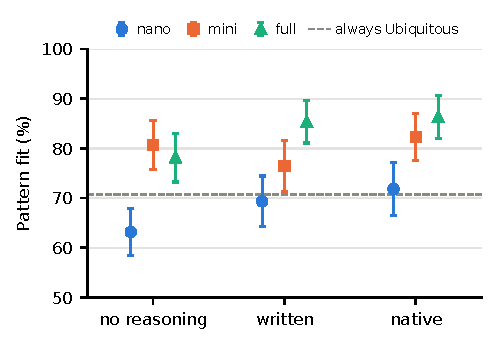
\includegraphics[width=\linewidth]{figures/study2b_fit_by_tier.pdf}
  \caption{Study 2 pattern fit by reasoning level and tier, averaged over examples and rules (600 outputs per point), with 95\% intervals over items. Dashed: constant-Ubiquitous baseline under the union (70.7\%). The axis starts at 50\%.}
  \Description{A line chart of pattern fit in percent (axis from 50 to 100) against reasoning level (none, written, native), one line per tier. Nano rises from about 63 to 69 to 72 percent. Mini goes from about 81 to 77 to 82 percent. The full tier rises from about 78 to 85 to 86 percent. A dashed horizontal line marks the constant-Ubiquitous baseline at 70.7 percent.}
  \label{fig:2b-tier}
\end{figure}

\subsection{RQ3: What a form-only checker misses (Study~1, exploratory)}
\label{sec:results-formfit}

% Generated by study2/scripts/make_paper_results.py from the committed analysis outputs.
% Do not edit by hand: change the script and re-run it.
Scored by the checker, Study~1's base prompt already reaches 86.7\% to 95.3\% across tiers (Table~\ref{tab:study1}). Examples add +2.6 pp [1.2, 4.0] ($p_{\mathrm{Holm}}=.001$) and rules +2.7 pp [0.6, 4.8] ($p_{\mathrm{Holm}}=.059$, no difference detected); no ingredient $\times$ tier test is significant. The largest difference is the base prompt over the Name-only prompt, +19.1 pp [15.0, 23.2] ($p_{\mathrm{Holm}}<.001$); JSON output makes no detectable difference (0.0 pp).

% Generated by study2/scripts/make_paper_results.py from the committed analysis outputs.
% Do not edit by hand: change the script and re-run it.
The checker accepts any opening WHERE clause. Without examples, nano uses WHERE in 63 to 76 of 150 outputs per factorial condition (Table~\ref{tab:study1}; 43 with the JSON prompt), and with examples in 6 to 9. The larger tiers use it in 9 to 26 outputs without examples (post hoc counts). Only one of the 150 source requirements opens with ``Where''; Fig.~\ref{fig:example} shows one such output.


% Generated by study2b/scripts/make_paper_results_2b.py.
\begin{table}
  \caption{Study 1 by condition: checker compliance and pattern fit (union labels) per tier, in \%, and the number of nano outputs, of 150, that use WHERE. Base = base prompt; +E, +C and +R add examples, the chain-of-thought sentence and rules.}
  \label{tab:study1}
  \footnotesize
  \setlength{\tabcolsep}{3pt}
  \begin{tabular}{@{}lccccccc@{}}
    \toprule
    & \multicolumn{3}{c}{Checker} & \multicolumn{3}{c}{Pattern fit} & WHERE \\
    \cmidrule(lr){2-4}\cmidrule(lr){5-7}\cmidrule(l){8-8}
    Condition & nano & mini & full & nano & mini & full & nano \\
    \midrule
    Name-only & 56.0 & 78.7 & 82.7 & 54.0 & 63.3 & 73.3 & 0 \\
    Base & 86.7 & 92.7 & 95.3 & 47.3 & 72.7 & 60.0 & 63 \\
    \midrule
    Base+E & 90.0 & 96.7 & 98.0 & 78.0 & 83.3 & 84.7 & 9 \\
    Base+C & 82.7 & 92.7 & 96.7 & 39.3 & 78.0 & 65.3 & 73 \\
    Base+R & 94.7 & 92.0 & 98.0 & 46.0 & 79.3 & 74.7 & 73 \\
    Base+EC & 89.3 & 96.0 & 98.0 & 78.0 & 84.0 & 86.7 & 9 \\
    Base+ER & 91.3 & 97.3 & 99.3 & 82.7 & 85.3 & 90.7 & 6 \\
    Base+CR & 93.3 & 91.3 & 99.3 & 40.7 & 80.0 & 76.0 & 76 \\
    Base+ECR & 94.0 & 97.3 & 99.3 & 85.3 & 86.0 & 88.7 & 6 \\
    \midrule
    JSON & 88.7 & 92.0 & 94.0 & 42.7 & 72.7 & 54.0 & 43 \\
    \bottomrule
  \end{tabular}
\end{table}


We then re-scored Study~1 with Study~2's labels, a secondary analysis fixed in Study~2's plan after Study~1's outputs had been inspected. The base prompt's advantage over the Name-only prompt is then no longer detected: $-$3.6 pp ($p=.30$, unadjusted) instead of +19.1 pp (per label set in Table~\ref{tab:labelsets}, per-tier rates in Table~\ref{tab:study1}). Worked examples raise pattern fit by +21.2 pp ($p_{\mathrm{Holm}}<.001$), against +2.6 pp for checker compliance, and rules by +4.8 pp ($p_{\mathrm{Holm}}=.002$). Base+R gave nano its highest checker compliance (94.7\%) but a pattern fit of 46.0\%. The pattern that the JSON prompt makes the model name matches its opening keyword in all 412 compliant outputs, so the model's own label cannot reveal a wrong choice (post hoc).

\subsection{Where the gains come from (post hoc)}
\label{sec:results-posthoc}

These analyses were added after the planned ones (Table~\ref{tab:protocol}). Most pattern-fit gains come from outputs that no longer add a condition the input does not state. Worked examples raise checker compliance only from 93.4\% to 95.4\%, but the share of Ubiquitous outputs from 42.5\% to 57.4\%. Table~\ref{tab:strata} splits the inputs by admissible set. On the 68 inputs for which only Ubiquitous is admissible, every ingredient helps. On the 44 inputs that require a condition, pattern fit is already high (78.8\% for the base prompt), and only native reasoning, of the four Study~2 contrasts, helps detectably. Study~1's base prompt raises pattern fit on the inputs that require a condition and lowers it on the Ubiquitous-only ones, where the Name-only prompt mostly writes unconditional requirements (72.0\% of its nano outputs). On the 100 inputs whose best pattern both annotators agree on, outputs for Ubiquitous inputs use WHERE in 9.3\% and WHEN in 7.8\% of cases, while event-driven and unwanted-behaviour inputs get their pattern in 80.3\% and 88.4\%. Reasoning adds less when examples are present (examples $\times$ written $-$8.1 pp; examples $\times$ native $-$9.7 pp), whereas rules and native reasoning reinforce each other (+7.4 pp); all three intervals exclude zero.

% Generated by study2b/scripts/make_paper_results_2b.py.
\begin{table*}
  \caption{Post hoc: effects on pattern fit by input stratum, in percentage points with 95\% intervals (item-level paired differences, unadjusted). Strata come from the union admissible sets. The Study~2 columns average over the other factors and the three tiers; the last column is Study~1's Base minus Name-only. For all inputs the estimates equal the planned GEE estimates; the intervals use a $t$ reference.}
  \label{tab:strata}
  \footnotesize
  \setlength{\tabcolsep}{2.5pt}
  \begin{tabular}{@{}lrccccc@{}}
    \toprule
    & & \multicolumn{4}{c}{Study 2} & Study 1 \\
    \cmidrule(lr){3-6}\cmidrule(l){7-7}
    Inputs & $n$ & Examples & Rules & Written $-$ none & Native $-$ none & Base $-$ Name-only \\
    \midrule
    A condition is required & 44 & +1.8 [$-$2.2, 5.7] & +1.3 [$-$4.5, 7.0] & $-$4.4 [$-$9.2, 0.5] & +6.8 [2.9, 10.8] & +17.4 [6.4, 28.5] \\
    Only Ubiquitous admissible & 68 & +17.8 [14.2, 21.4] & +9.0 [5.1, 12.9] & +8.7 [5.0, 12.4] & +7.0 [2.5, 11.5] & $-$23.0 [$-$32.6, $-$13.5] \\
    Mixed & 38 & +9.4 [4.2, 14.6] & +6.4 [1.8, 11.0] & +1.5 [$-$3.0, 6.1] & +3.9 [$-$1.3, 9.1] & +7.0 [$-$5.8, 19.8] \\
    \midrule
    All inputs & 150 & +11.0 [8.4, 13.5] & +6.1 [3.4, 8.8] & +3.1 [0.5, 5.6] & +6.2 [3.5, 8.8] & $-$3.6 [$-$10.4, 3.3] \\
    \bottomrule
  \end{tabular}
\end{table*}


Both annotators had rated Study~1 outputs for 50 inputs. On the other 100, the Study~2 effects keep their size (examples +10.9, rules +5.0, written +4.4, native +5.8 pp, all above zero). By contrast, Study~1's Base-versus-Name-only estimate is +0.3 pp [$-$8.5, 9.1] on them and $-$11.3 pp on the 50 rated inputs. Within Study~1, the inert step-by-step sentence acts as a placebo: it changes pattern fit by +0.3 pp [$-$1.0, 1.6].

\subsection{Human ratings (exploratory)}
\label{sec:results-2b-human}

R1 and R2 rated 150 base-prompt outputs (17, 17 and 16 items on nano, mini and full). Agreement is low. Across the five criteria, the highest Krippendorff's $\alpha$ is 0.50 (Singularity) and the lowest $-$0.56 (Unambiguity); quadratic-weighted $\kappa$ lies between $-$0.04 and 0.42, and exact and within-one agreement exceed chance by at most 11 and 6 points. Low agreement is common when humans rate requirement quality: among five evaluators, Paiva et al.~\cite{paiva2026issuetitles} report $\alpha$ between 0.150 and 0.394. Ours is lower still on two criteria. Scores sit near the ceiling (every condition mean at least 4.30; 91\% of outputs have a mean equivalence of at least 4), and no difference between reasoning levels is Holm-significant (smallest $p_{\mathrm{Holm}}=.233$), also for R2 alone. Post hoc, the checker's 14 non-compliant outputs received lower EARS well-formedness scores (4.57 vs 4.92). Outputs with pattern fit received higher equivalence scores (4.80 vs 4.41), but this difference comes from R1 (+0.64 [0.30, 0.98]), who is also an annotator, and is not detected for R2 (+0.12 [$-$0.11, 0.35]).
